% Options for packages loaded elsewhere
\PassOptionsToPackage{unicode}{hyperref}
\PassOptionsToPackage{hyphens}{url}
%
\documentclass[
  12pt,
]{article}
\title{Groundwater Recharge and Quality Analysis}
\usepackage{etoolbox}
\makeatletter
\providecommand{\subtitle}[1]{% add subtitle to \maketitle
  \apptocmd{\@title}{\par {\large #1 \par}}{}{}
}
\makeatother
\subtitle{\url{https://github.com/katieelliott98/WDA_Final.git}}
\author{Kaitlyn Elliott}
\date{}

\usepackage{amsmath,amssymb}
\usepackage{lmodern}
\usepackage{iftex}
\ifPDFTeX
  \usepackage[T1]{fontenc}
  \usepackage[utf8]{inputenc}
  \usepackage{textcomp} % provide euro and other symbols
\else % if luatex or xetex
  \usepackage{unicode-math}
  \defaultfontfeatures{Scale=MatchLowercase}
  \defaultfontfeatures[\rmfamily]{Ligatures=TeX,Scale=1}
  \setmainfont[]{Times New Roman}
\fi
% Use upquote if available, for straight quotes in verbatim environments
\IfFileExists{upquote.sty}{\usepackage{upquote}}{}
\IfFileExists{microtype.sty}{% use microtype if available
  \usepackage[]{microtype}
  \UseMicrotypeSet[protrusion]{basicmath} % disable protrusion for tt fonts
}{}
\makeatletter
\@ifundefined{KOMAClassName}{% if non-KOMA class
  \IfFileExists{parskip.sty}{%
    \usepackage{parskip}
  }{% else
    \setlength{\parindent}{0pt}
    \setlength{\parskip}{6pt plus 2pt minus 1pt}}
}{% if KOMA class
  \KOMAoptions{parskip=half}}
\makeatother
\usepackage{xcolor}
\IfFileExists{xurl.sty}{\usepackage{xurl}}{} % add URL line breaks if available
\IfFileExists{bookmark.sty}{\usepackage{bookmark}}{\usepackage{hyperref}}
\hypersetup{
  pdftitle={Groundwater Recharge and Quality Analysis},
  pdfauthor={Kaitlyn Elliott},
  hidelinks,
  pdfcreator={LaTeX via pandoc}}
\urlstyle{same} % disable monospaced font for URLs
\usepackage[margin=2.54cm]{geometry}
\usepackage{longtable,booktabs,array}
\usepackage{calc} % for calculating minipage widths
% Correct order of tables after \paragraph or \subparagraph
\usepackage{etoolbox}
\makeatletter
\patchcmd\longtable{\par}{\if@noskipsec\mbox{}\fi\par}{}{}
\makeatother
% Allow footnotes in longtable head/foot
\IfFileExists{footnotehyper.sty}{\usepackage{footnotehyper}}{\usepackage{footnote}}
\makesavenoteenv{longtable}
\usepackage{graphicx}
\makeatletter
\def\maxwidth{\ifdim\Gin@nat@width>\linewidth\linewidth\else\Gin@nat@width\fi}
\def\maxheight{\ifdim\Gin@nat@height>\textheight\textheight\else\Gin@nat@height\fi}
\makeatother
% Scale images if necessary, so that they will not overflow the page
% margins by default, and it is still possible to overwrite the defaults
% using explicit options in \includegraphics[width, height, ...]{}
\setkeys{Gin}{width=\maxwidth,height=\maxheight,keepaspectratio}
% Set default figure placement to htbp
\makeatletter
\def\fps@figure{htbp}
\makeatother
\setlength{\emergencystretch}{3em} % prevent overfull lines
\providecommand{\tightlist}{%
  \setlength{\itemsep}{0pt}\setlength{\parskip}{0pt}}
\setcounter{secnumdepth}{5}
\ifLuaTeX
  \usepackage{selnolig}  % disable illegal ligatures
\fi

\begin{document}
\maketitle

\newpage
\tableofcontents
\newpage

\hypertarget{rationale-and-rearch-questions}{%
\section{Rationale and Rearch
Questions}\label{rationale-and-rearch-questions}}

Knowing how precipitation affects groundwater levels is important for
managing groundwater extraction, especially with climate change and
changing rainfall distributions. Also knowing the likely quality of
water for a given groundwater depth can help inform decision making.
Given the importance of these factors, the focus of this projectn is to
understand the lag time between precipitation, stormflow is used as a
proxy, and groundwater levels. In reality this is trying to understand
the recharge time of the groundwater aquifer. Two different sites will
be analysed to see if there is a noticeable difference with different
geologies. The first site is in Houserville, PA and is Pennsylvanian
aquifer and the second is in Sewickley, PA and is a Valley and Ridge
aquifer. The second main question investigated is how water quality of
these aquifers has change overtime and how it changes with groundwater
level.

The Main Questions Analyzed

\begin{enumerate}
\def\labelenumi{\arabic{enumi}.}
\tightlist
\item
  How is groundwater levels and stormflow changing overtime? Is there
  seasonality?
\item
  How does storm flow impact groundwater levels?
\item
  How is groundwater quality changing overtime? Are chemicals more
  concentrated at low groundwater levels or high?
\end{enumerate}

\newpage

\hypertarget{dataset-information}{%
\section{Dataset Information}\label{dataset-information}}

All data used in this project is from the USGS. Datasets were picked
based on differing geology. First groundwater monitoring stations were
selected that had both water level data and water quality data. Then the
nearest stream gage with the most complete data was selected. Stream
flow was separated with lfstat into baseflow and stormflow. Stormflow in
this analysis is a proxy for precipitation because precipitation gage
information was hard to find near groundwater monitoring stations.

Table 1. Data Information for Project

\begin{longtable}[]{@{}llll@{}}
\toprule
Dataset & Variable & Unit & Source \\
\midrule
\endhead
Groundwater Level & Water Level & ft below surface & USGS \\
Groundwater Quality & pH & Standard Units & USGS \\
Gage Data & Discharge & ft\^{}3/s & USGS \\
All & Date & Y-m-d & USGS \\
\bottomrule
\end{longtable}

\newpage

\hypertarget{exploratory-analysis}{%
\section{Exploratory Analysis}\label{exploratory-analysis}}

A line plot was created with ggplot to get a view of the data. Figure 1
shows data for Houserville, PA, which exhibits very clear seasonal
patterns in the groundwater levels, and possibly seasonality for
stormflow. Figure 2 demonstrates the data for Sewickley, PA, which has
obvious seasonality in stormflow and is not clear on seasonality for
groundwater levels. Neither dataset has obvious trends overtime for
groundwater nor stormflow. Based on the exploratory analysis a good next
step would be a seasonal Mann-Kenall test to see if there is a trend
overtime and if there is strong statistical seasonality.

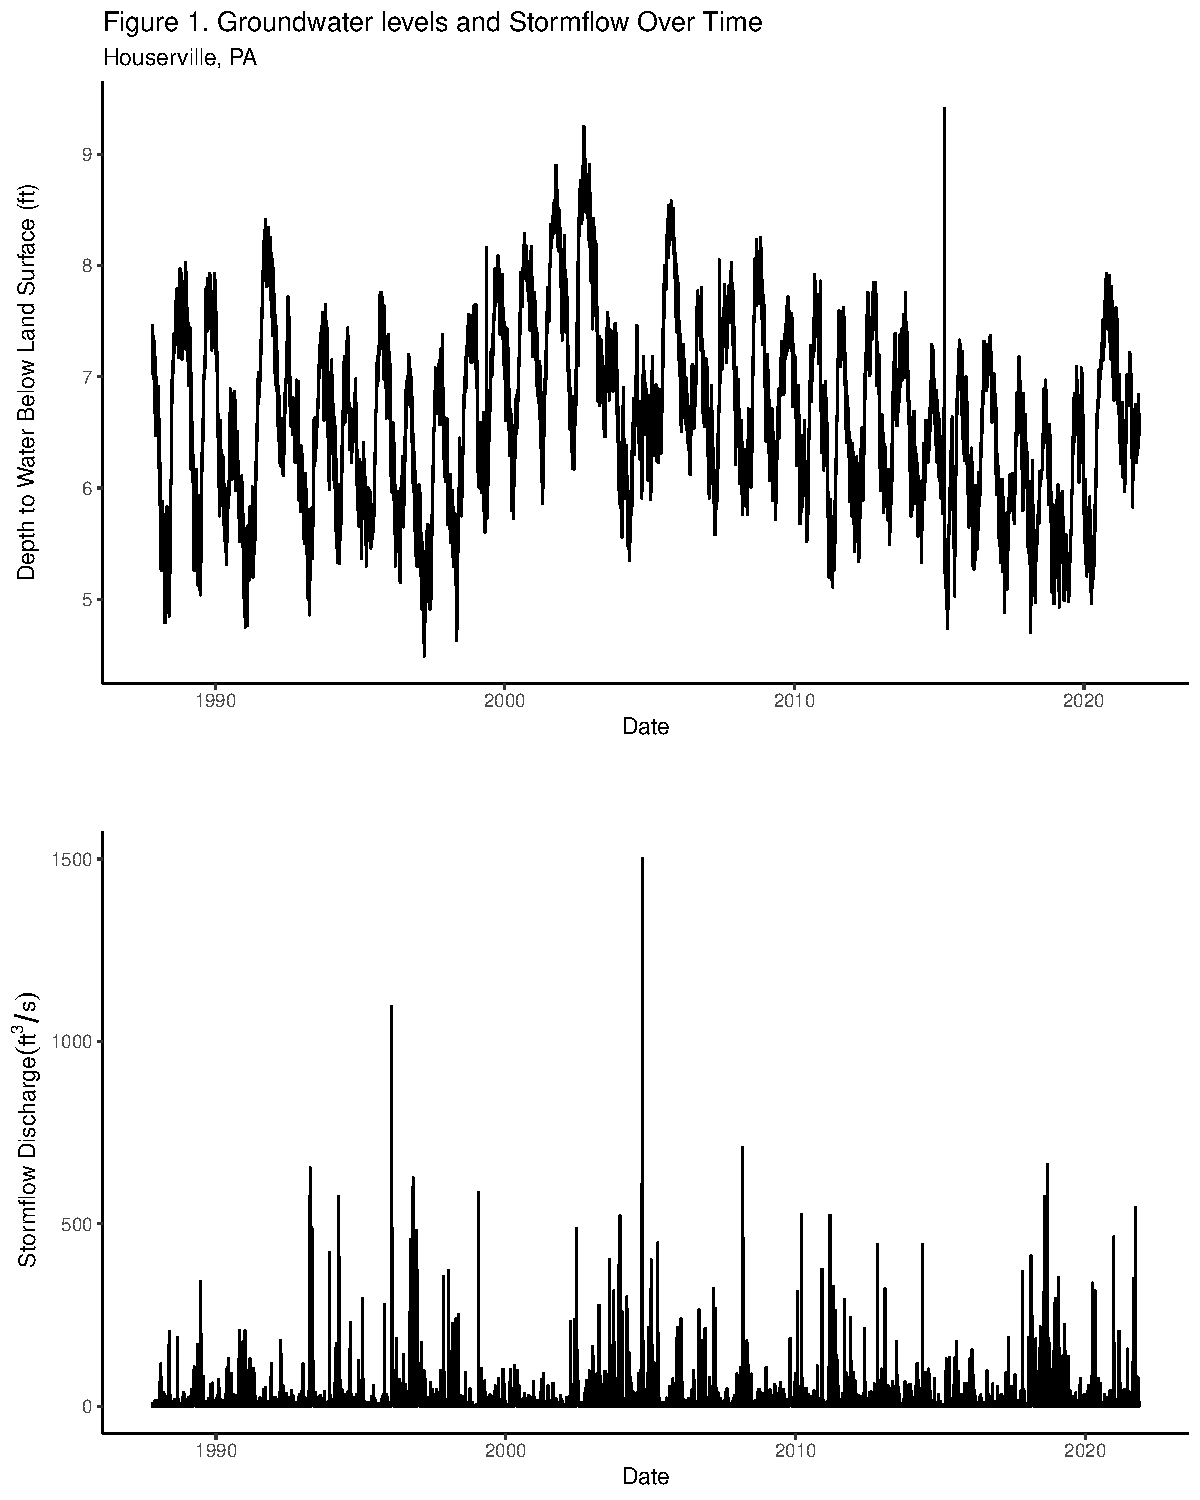
\includegraphics{Draft_Final_files/figure-latex/explore-1.pdf}
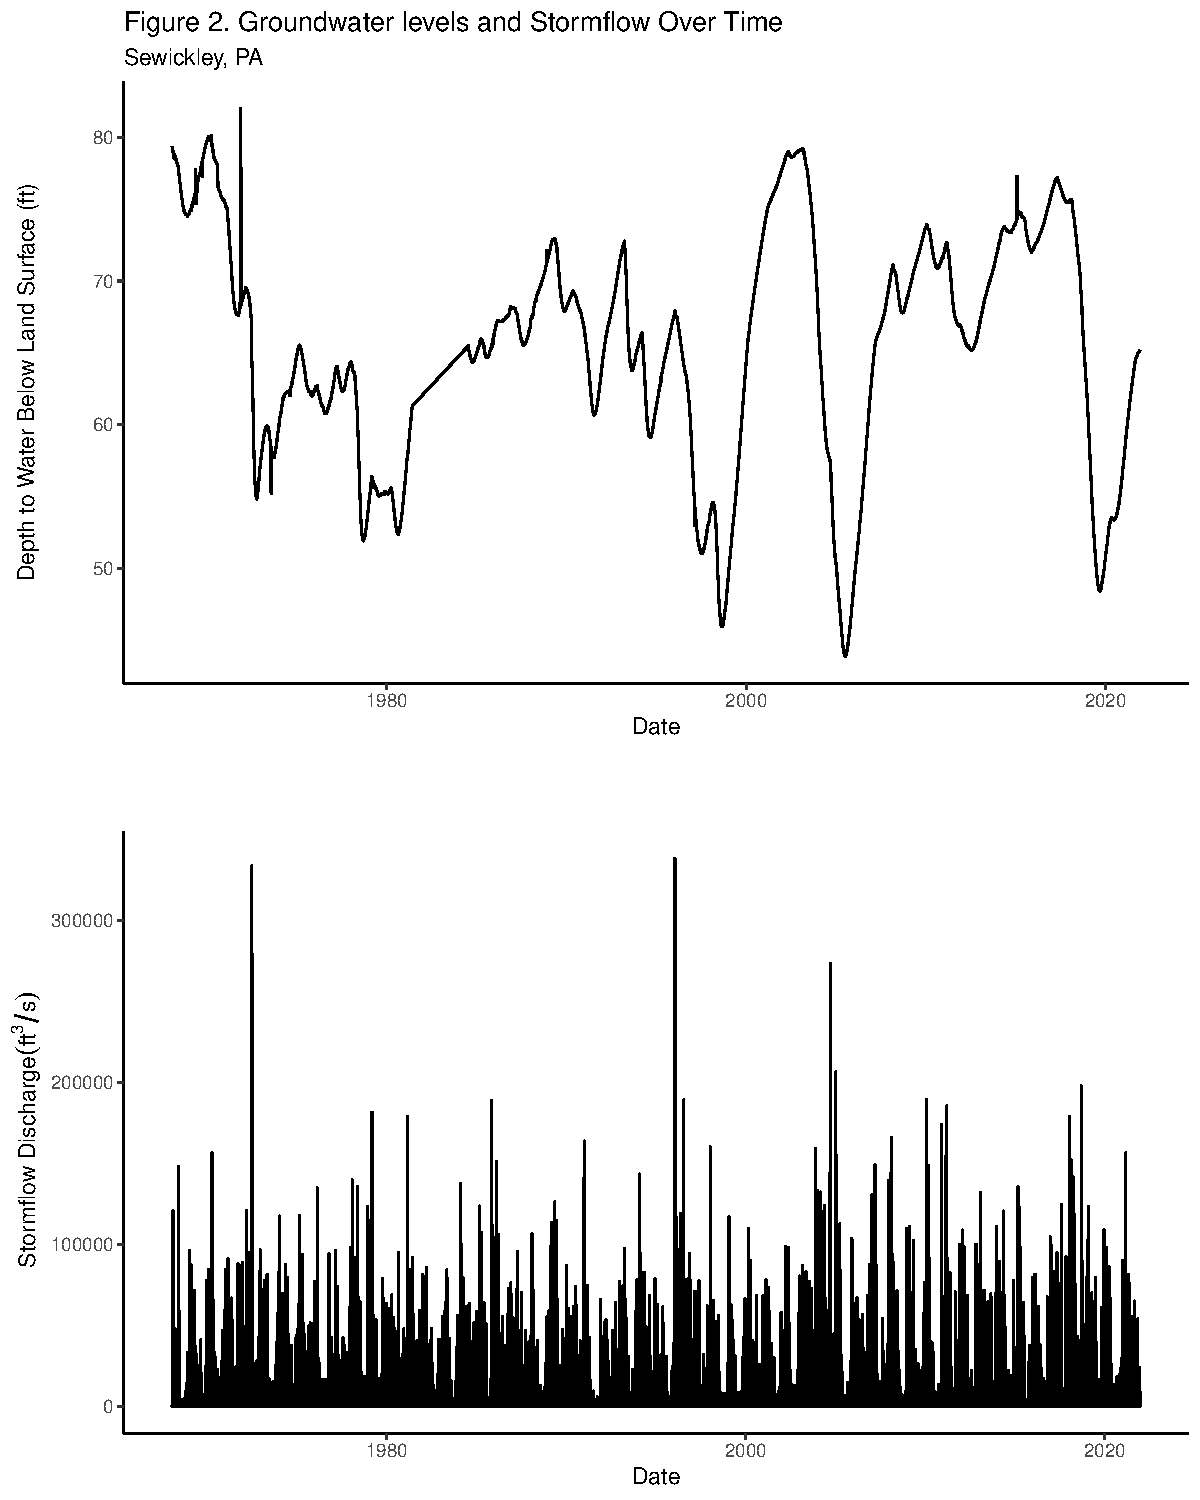
\includegraphics{Draft_Final_files/figure-latex/explore-2.pdf}

\newpage

\hypertarget{analysis}{%
\section{Analysis}\label{analysis}}

\hypertarget{question-1-how-is-groundwater-levels-and-stormflow-changing-overtime-is-there-seasonality}{%
\subsection{Question 1: How is groundwater levels and stormflow changing
overtime? Is there
seasonality?}\label{question-1-how-is-groundwater-levels-and-stormflow-changing-overtime-is-there-seasonality}}

Seasonality was analyzed for both groundwater levels and stormflow by
first aggregating the datasets into monthly data. Then they were
transformed into time series and decomposed. The results of this can be
seen in Figures 1234. Then a seasonal Mann-Kendall test was run based on
the presence of seasonality. The results of these tests showed the
overall trend overtime in both Houserville and Sewickley, PA for their
groundwater levels and their stormflow.

\hypertarget{decomposition-and-trend-analysis-for-houserville-pa-stormflow}{%
\subsubsection{Decomposition and Trend Analysis for Houserville, PA:
Stormflow}\label{decomposition-and-trend-analysis-for-houserville-pa-stormflow}}

There is a seasonal trend for stormflow in Houserville, PA. So the
Mann-Kendall test was run producing a z value of -3.8953 and a p-value
of 0.00009809. Meaning that it is statistically significant that
stormflow is trending downward over time.

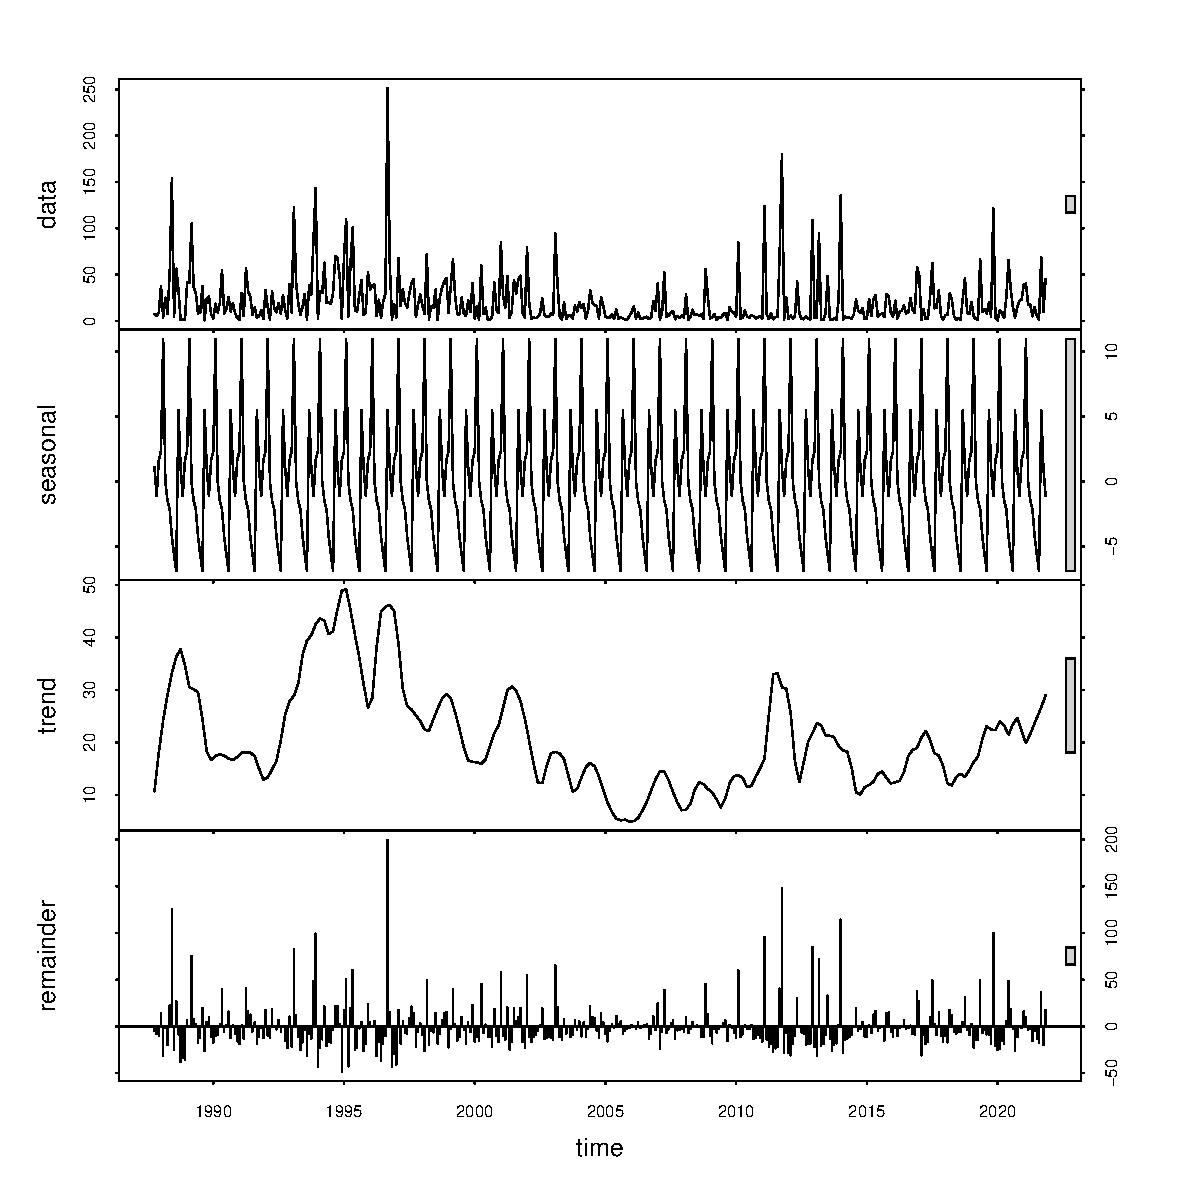
\includegraphics{Draft_Final_files/figure-latex/seasonality-1.pdf}

\begin{verbatim}
## 
##  Seasonal Mann-Kendall trend test (Hirsch-Slack test)
## 
## data:  penn_gage_ts
## z = -3.8953, p-value = 0.00009809
## alternative hypothesis: true S is not equal to 0
## sample estimates:
##     S  varS 
##  -918 55420
\end{verbatim}

\begin{verbatim}
## 
##  Seasonal Mann-Kendall trend test (Hirsch-Slack test)
## 
## data: penn_gage_ts
## alternative hypothesis: two.sided
## 
## Statistics for individual seasons
## 
## H0
##                       S   varS    tau      z  Pr(>|z|)   
## Season 1:   S = 0   -41 4550.3 -0.073 -0.593 0.5531961   
## Season 2:   S = 0  -137 4550.3 -0.244 -2.016 0.0437870  *
## Season 3:   S = 0   -97 4550.3 -0.173 -1.423 0.1546937   
## Season 4:   S = 0  -183 4550.3 -0.326 -2.698 0.0069747 **
## Season 5:   S = 0  -131 4550.3 -0.234 -1.927 0.0539575  .
## Season 6:   S = 0   -93 4550.3 -0.166 -1.364 0.1726152   
## Season 7:   S = 0   -29 4550.3 -0.052 -0.415 0.6780801   
## Season 8:   S = 0  -171 4550.3 -0.305 -2.520 0.0117303  *
## Season 9:   S = 0   -57 4550.3 -0.102 -0.830 0.4064433   
## Season 10:   S = 0   -9 4958.3 -0.015 -0.114 0.9095458   
## Season 11:   S = 0   31 4958.3  0.052  0.426 0.6700765   
## Season 12:   S = 0   -1 4550.3 -0.002  0.000 1.0000000   
## ---
## Signif. codes:  0 '***' 0.001 '**' 0.01 '*' 0.05 '.' 0.1 ' ' 1
\end{verbatim}

\newpage

\hypertarget{decomposition-and-trend-analysis-for-houserville-pa-groundwater}{%
\subsubsection{Decomposition and Trend Analysis for Houserville, PA:
Groundwater}\label{decomposition-and-trend-analysis-for-houserville-pa-groundwater}}

There is a seasonal trend for groundwater levels in Houserville, PA. So
the Mann-Kendall test was run producing a z value of 9.4939 and a
p-value of \textless{} 2.2e-16. Meaning that it is statistically
significant that distance from the surface to the groundwater level is
trending upward over time. This suggests ground water is decreasing over
time.

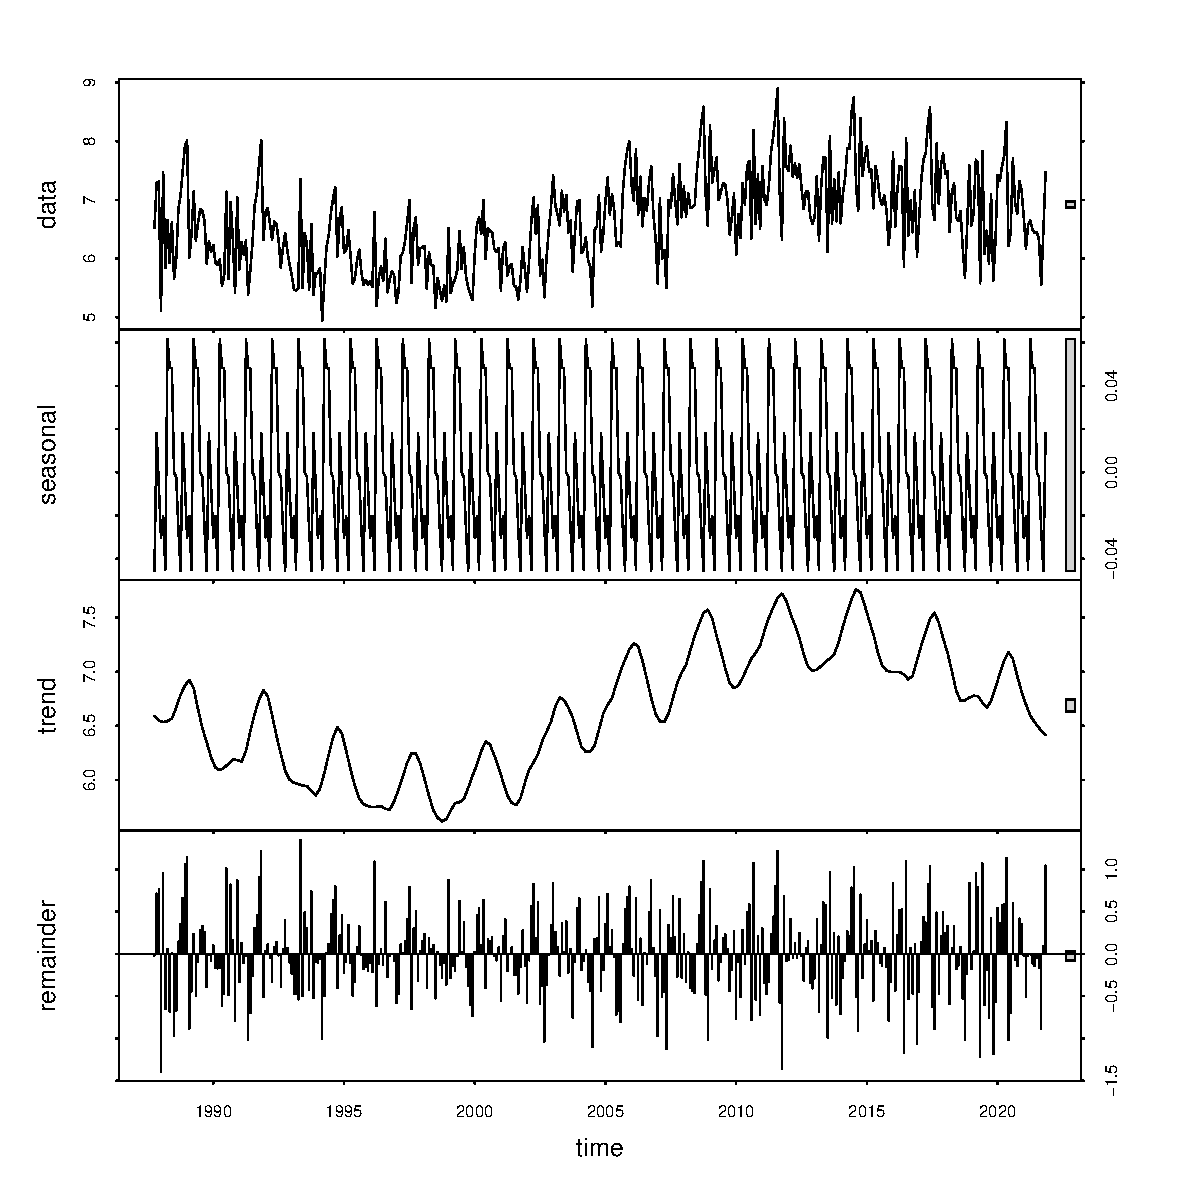
\includegraphics{Draft_Final_files/figure-latex/seasonality_2-1.pdf}

\begin{verbatim}
## 
##  Seasonal Mann-Kendall trend test (Hirsch-Slack test)
## 
## data:  penn_aqu_ts
## z = 9.4939, p-value < 2.2e-16
## alternative hypothesis: true S is not equal to 0
## sample estimates:
##     S  varS 
##  2236 55420
\end{verbatim}

\begin{verbatim}
## 
##  Seasonal Mann-Kendall trend test (Hirsch-Slack test)
## 
## data: penn_aqu_ts
## alternative hypothesis: two.sided
## 
## Statistics for individual seasons
## 
## H0
##                      S   varS   tau     z    Pr(>|z|)    
## Season 1:   S = 0  181 4550.3 0.323 2.668  0.00762135  **
## Season 2:   S = 0  223 4550.3 0.398 3.291  0.00099823 ***
## Season 3:   S = 0  267 4550.3 0.476 3.943 0.000080367 ***
## Season 4:   S = 0  291 4550.3 0.519 4.299 0.000017150 ***
## Season 5:   S = 0  257 4550.3 0.458 3.795  0.00014761 ***
## Season 6:   S = 0  235 4550.3 0.419 3.469  0.00052256 ***
## Season 7:   S = 0  127 4550.3 0.226 1.868  0.06177882   .
## Season 8:   S = 0  185 4550.3 0.330 2.728  0.00637781  **
## Season 9:   S = 0   71 4550.3 0.127 1.038  0.29940461    
## Season 10:   S = 0 113 4958.3 0.190 1.591  0.11170854    
## Season 11:   S = 0 151 4958.3 0.254 2.130  0.03315388   *
## Season 12:   S = 0 135 4550.3 0.241 1.986  0.04698056   *
## ---
## Signif. codes:  0 '***' 0.001 '**' 0.01 '*' 0.05 '.' 0.1 ' ' 1
\end{verbatim}

\newpage

\hypertarget{decomposition-and-trend-analysis-for-sewickley-pa-stormflow}{%
\subsubsection{Decomposition and Trend Analysis for Sewickley, PA:
Stormflow}\label{decomposition-and-trend-analysis-for-sewickley-pa-stormflow}}

There is a seasonal trend for stormflow in Sweickley, PA. So the
Mann-Kendall test was run producing a z value of -8.7502 and a p-value
of \textless{} 2.2 e-16. Meaning that it is statistically significant
that stormflow is trending downward over time.

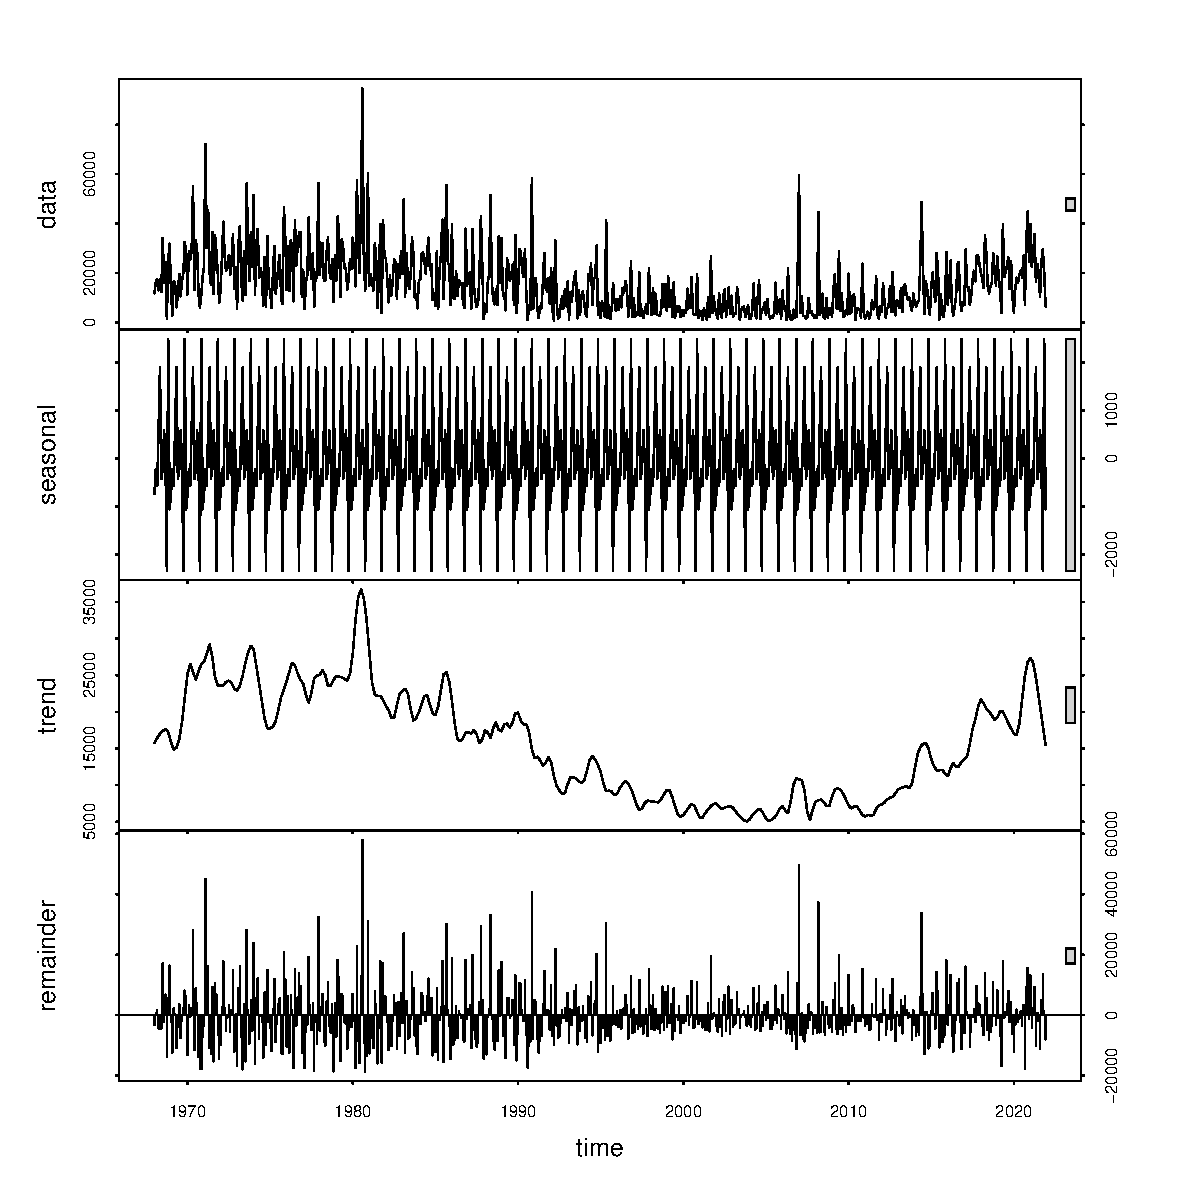
\includegraphics{Draft_Final_files/figure-latex/seasonality_3-1.pdf}

\begin{verbatim}
## 
##  Seasonal Mann-Kendall trend test (Hirsch-Slack test)
## 
## data:  vr_gage_ts
## z = -8.7502, p-value < 2.2e-16
## alternative hypothesis: true S is not equal to 0
## sample estimates:
##      S   varS 
##  -4064 215604
\end{verbatim}

\begin{verbatim}
## 
##  Seasonal Mann-Kendall trend test (Hirsch-Slack test)
## 
## data: vr_gage_ts
## alternative hypothesis: two.sided
## 
## Statistics for individual seasons
## 
## H0
##                       S  varS    tau      z   Pr(>|z|)    
## Season 1:   S = 0  -287 17967 -0.201 -2.134 0.03286940   *
## Season 2:   S = 0  -291 17967 -0.203 -2.164 0.03050148   *
## Season 3:   S = 0  -295 17967 -0.206 -2.193 0.02828159   *
## Season 4:   S = 0  -461 17967 -0.322 -3.432 0.00059962 ***
## Season 5:   S = 0  -317 17967 -0.222 -2.357 0.01839910   *
## Season 6:   S = 0  -233 17967 -0.163 -1.731 0.08348509   .
## Season 7:   S = 0  -479 17967 -0.335 -3.566 0.00036237 ***
## Season 8:   S = 0  -323 17967 -0.226 -2.402 0.01629460   *
## Season 9:   S = 0  -357 17967 -0.249 -2.656 0.00790964  **
## Season 10:   S = 0 -249 17967 -0.174 -1.850 0.06428766   .
## Season 11:   S = 0 -415 17967 -0.290 -3.089 0.00201098  **
## Season 12:   S = 0 -357 17967 -0.249 -2.656 0.00790964  **
## ---
## Signif. codes:  0 '***' 0.001 '**' 0.01 '*' 0.05 '.' 0.1 ' ' 1
\end{verbatim}

\newpage

\hypertarget{decomposition-and-trend-analysis-for-sewickley-pa-groundwater}{%
\subsubsection{Decomposition and Trend Analysis for Sewickley, PA:
Groundwater}\label{decomposition-and-trend-analysis-for-sewickley-pa-groundwater}}

There is a seasonal trend for groundwater level in Sewickley, PA. So the
Mann-Kendall test was run producing a z value of -0.56856 and a p-value
of 0.5697. This means that there is no statistically significant trend
over time.

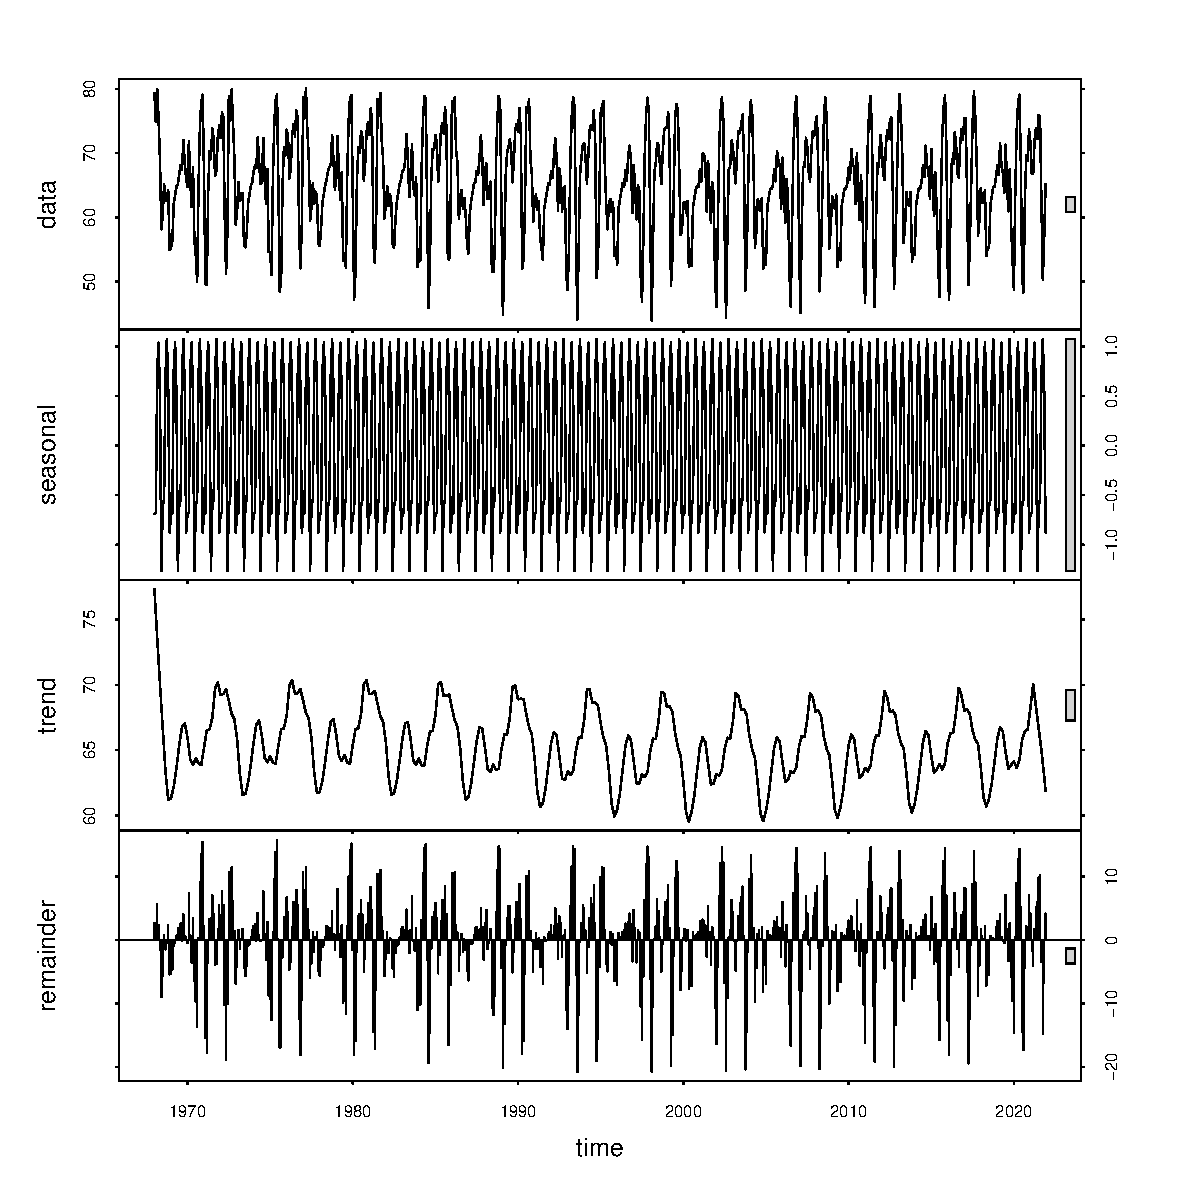
\includegraphics{Draft_Final_files/figure-latex/seasonality_4-1.pdf}

\begin{verbatim}
## 
##  Seasonal Mann-Kendall trend test (Hirsch-Slack test)
## 
## data:  vr_aqu_ts
## z = -0.56856, p-value = 0.5697
## alternative hypothesis: true S is not equal to 0
## sample estimates:
##      S   varS 
##   -265 215603
\end{verbatim}

\begin{verbatim}
## 
##  Seasonal Mann-Kendall trend test (Hirsch-Slack test)
## 
## data: vr_aqu_ts
## alternative hypothesis: two.sided
## 
## Statistics for individual seasons
## 
## H0
##                       S  varS    tau      z Pr(>|z|)  
## Season 1:   S = 0   -31 17967 -0.022 -0.224  0.82290  
## Season 2:   S = 0   -43 17967 -0.030 -0.313  0.75402  
## Season 3:   S = 0   -11 17967 -0.008 -0.075  0.94053  
## Season 4:   S = 0   138 17966  0.096  1.022  0.30673  
## Season 5:   S = 0  -101 17967 -0.071 -0.746  0.45564  
## Season 6:   S = 0    35 17967  0.024  0.254  0.79976  
## Season 7:   S = 0    31 17967  0.022  0.224  0.82290  
## Season 8:   S = 0   -21 17967 -0.015 -0.149  0.88139  
## Season 9:   S = 0   -51 17967 -0.036 -0.373  0.70913  
## Season 10:   S = 0   17 17967  0.012  0.119  0.90499  
## Season 11:   S = 0 -215 17967 -0.150 -1.597  0.11037  
## Season 12:   S = 0  -13 17967 -0.009 -0.090  0.92866  
## ---
## Signif. codes:  0 '***' 0.001 '**' 0.01 '*' 0.05 '.' 0.1 ' ' 1
\end{verbatim}

\newpage

\hypertarget{question-2-how-does-stormflow-impact-groundwater-levels}{%
\subsection{Question 2: How does stormflow impact groundwater
levels?}\label{question-2-how-does-stormflow-impact-groundwater-levels}}

To understand how stormflow impacts groundwater level the two datasets
were combined by date to consildate the information. Stormflow and
groundwater were plotting against each other to see if there was any
correlation, as seen in Figure 3 and 6. A CCF (cross correlation
function) was run to understand what lag leads to the best correlation
between the two variables. This test was run for both sites and was run
with and without seasonality included to see if there was a difference.
The results of the CCF were fairly inconclusive given what researchers
know about the relationship between groundwater and precipitation. CCF
figures are 4, 5, 7, and 8.

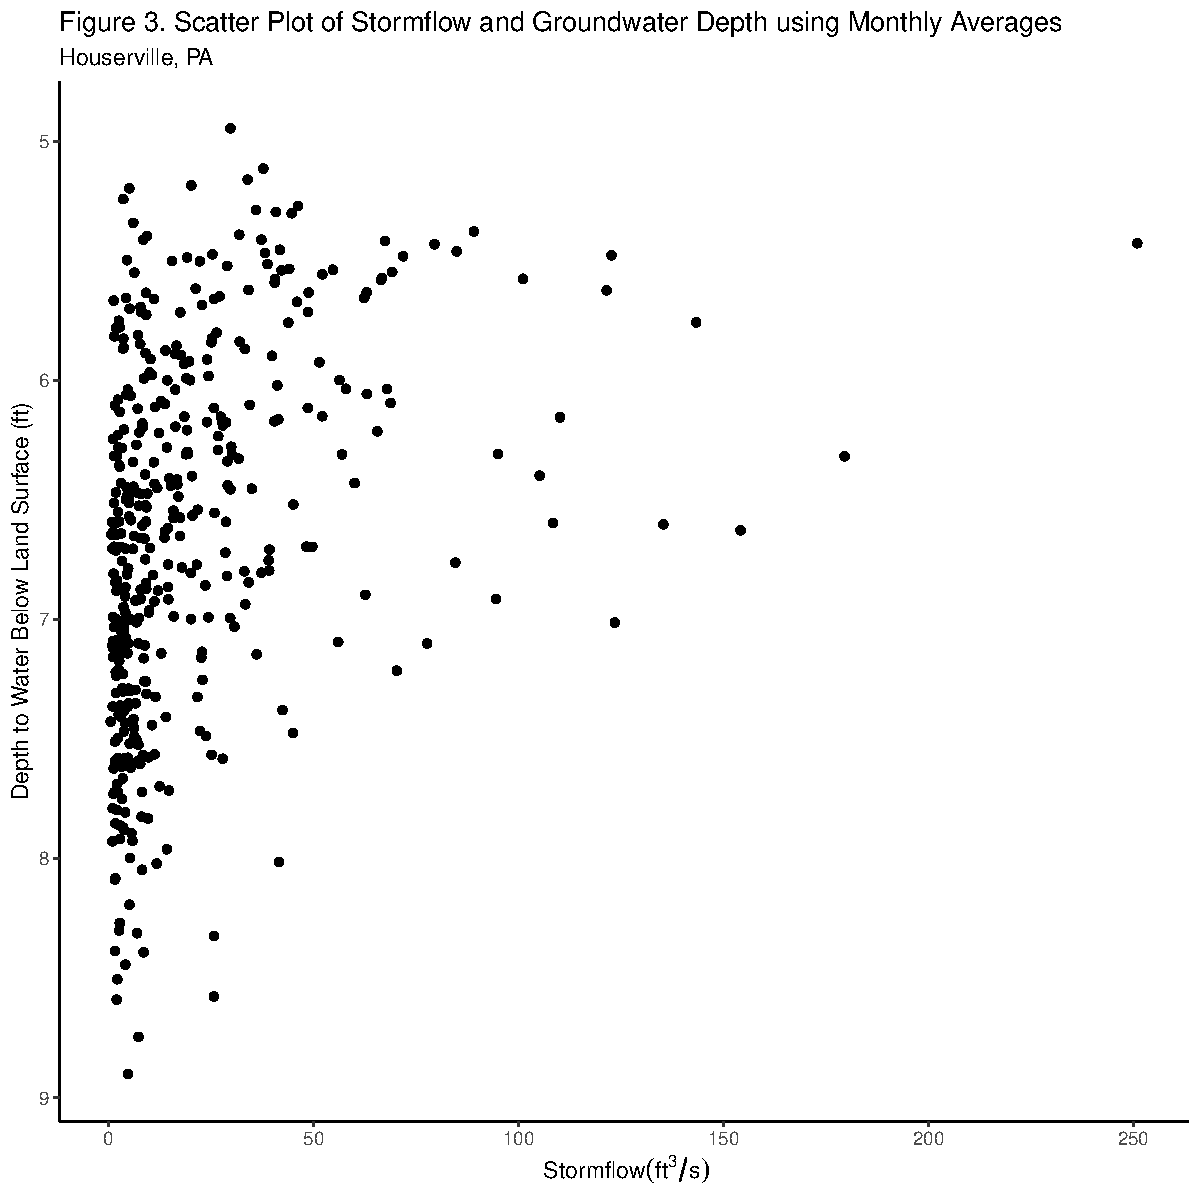
\includegraphics{Draft_Final_files/figure-latex/groundwater_lag-1.pdf}
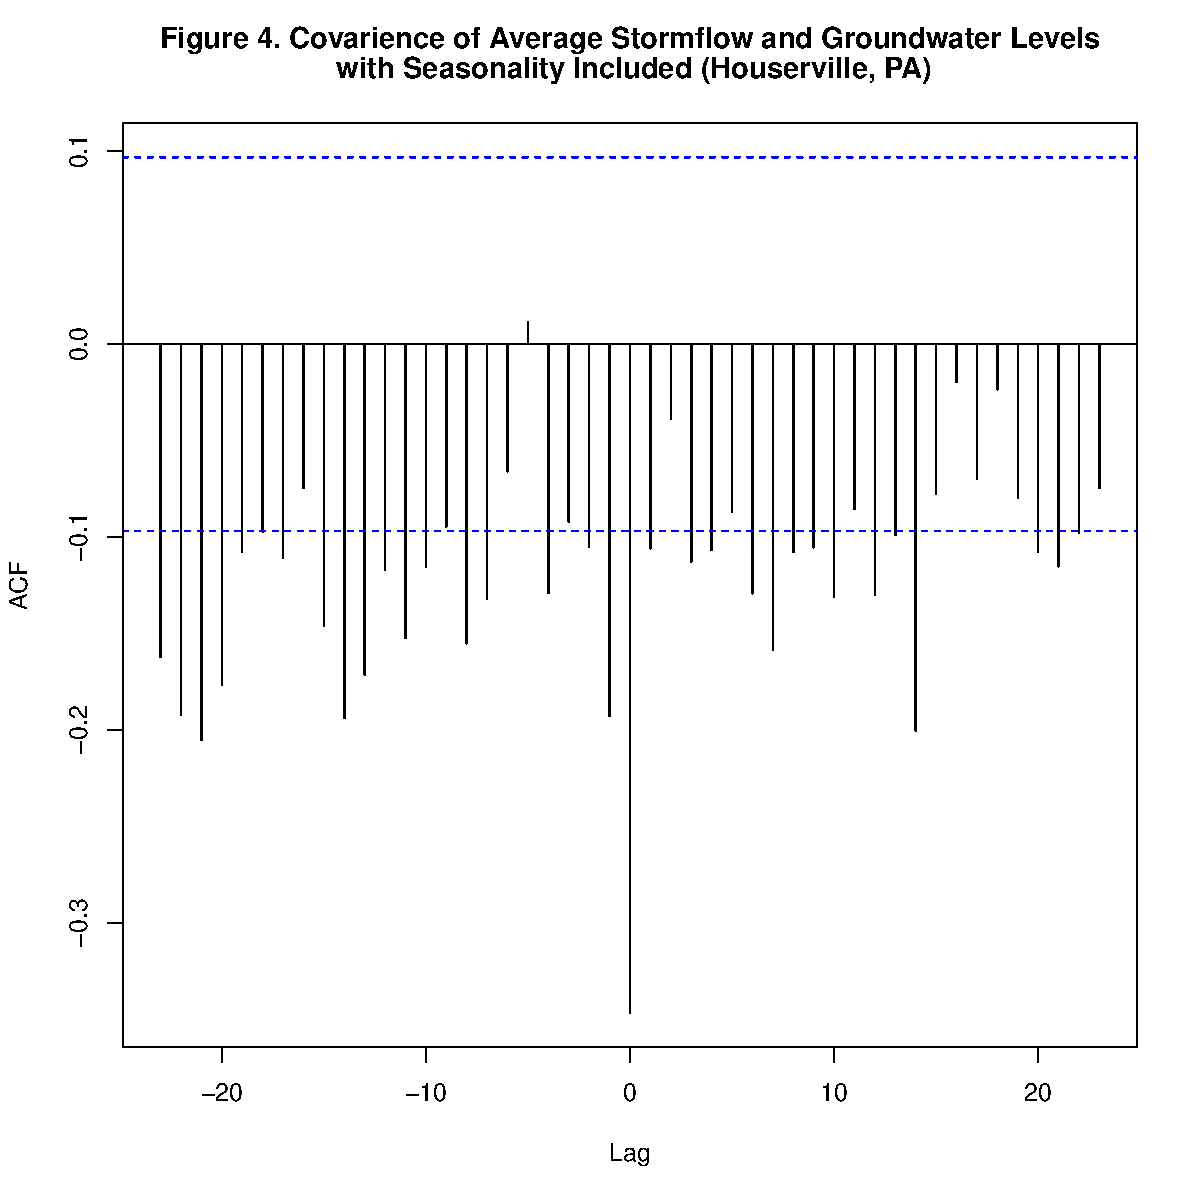
\includegraphics{Draft_Final_files/figure-latex/groundwater_lag-2.pdf}
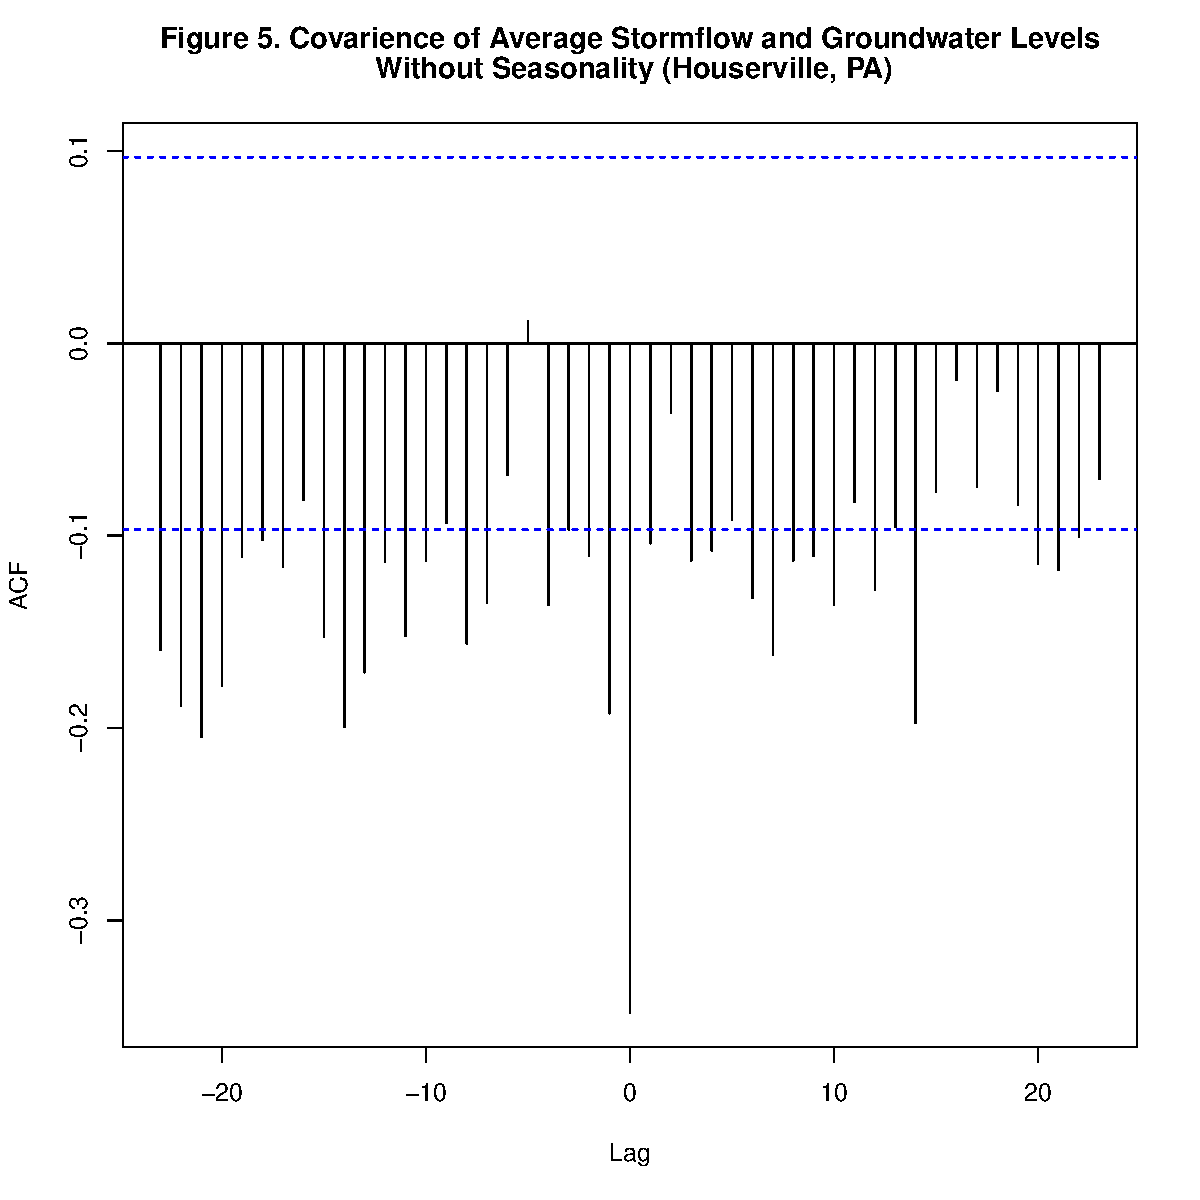
\includegraphics{Draft_Final_files/figure-latex/groundwater_lag-3.pdf}
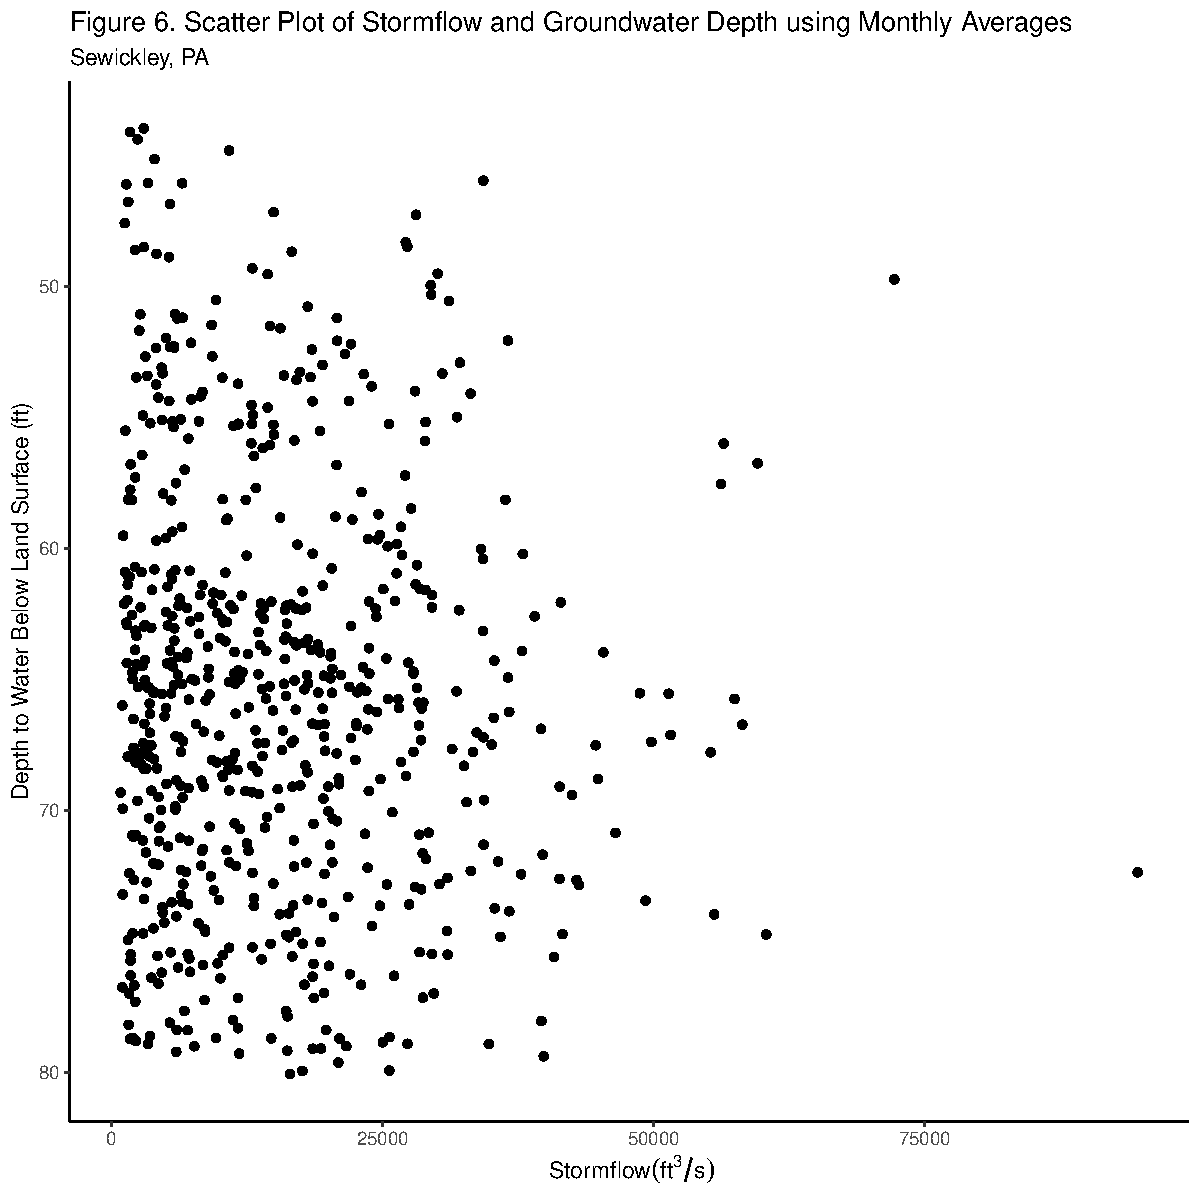
\includegraphics{Draft_Final_files/figure-latex/groundwater_lag-4.pdf}
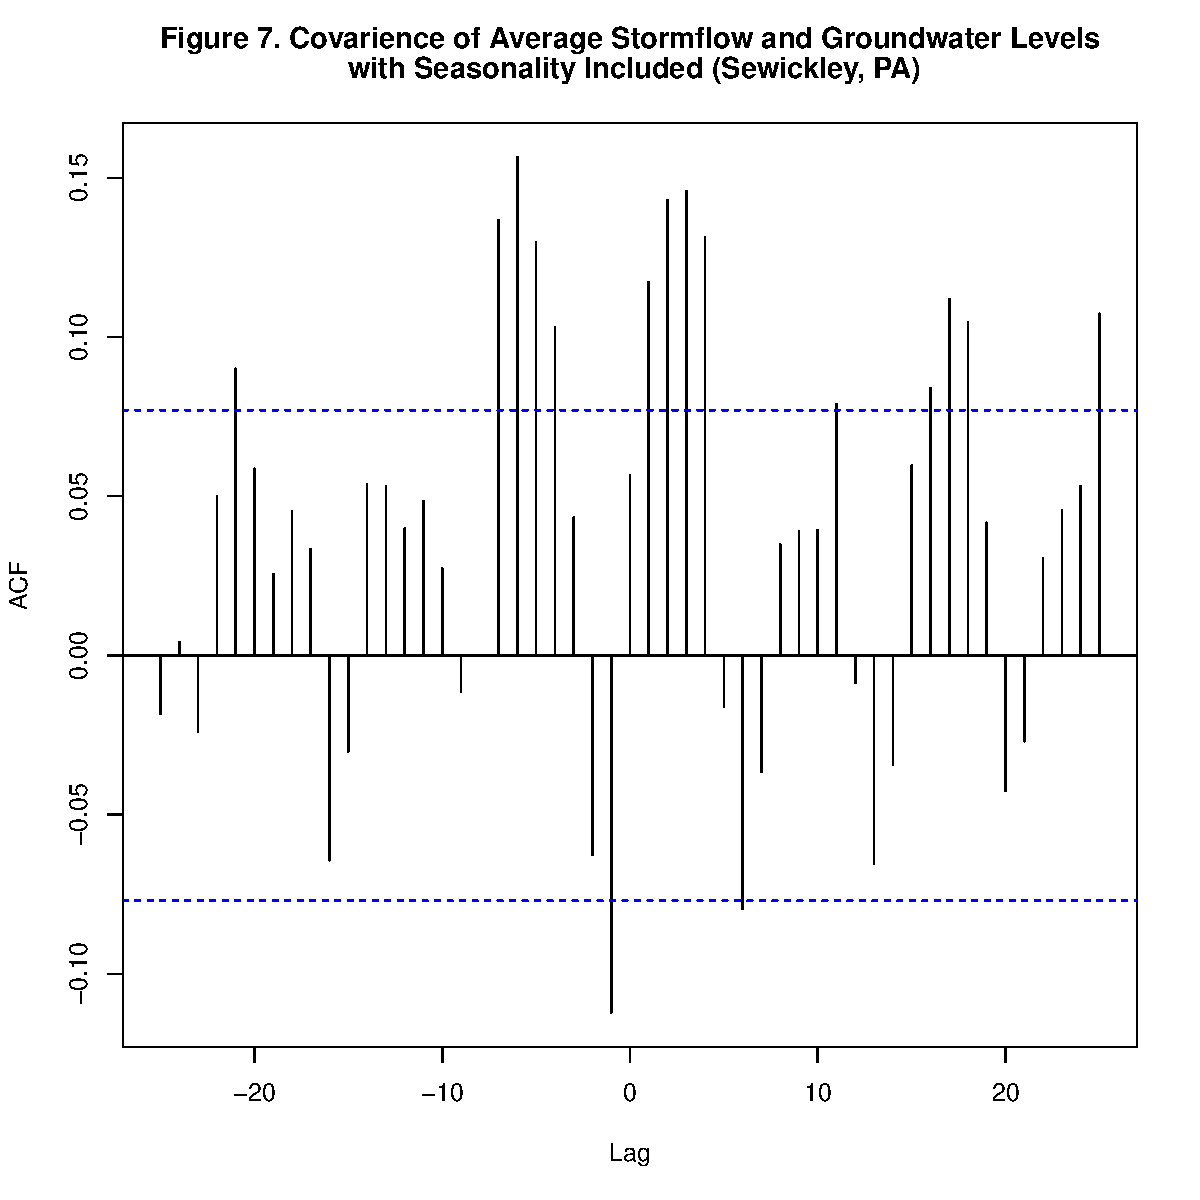
\includegraphics{Draft_Final_files/figure-latex/groundwater_lag-5.pdf}
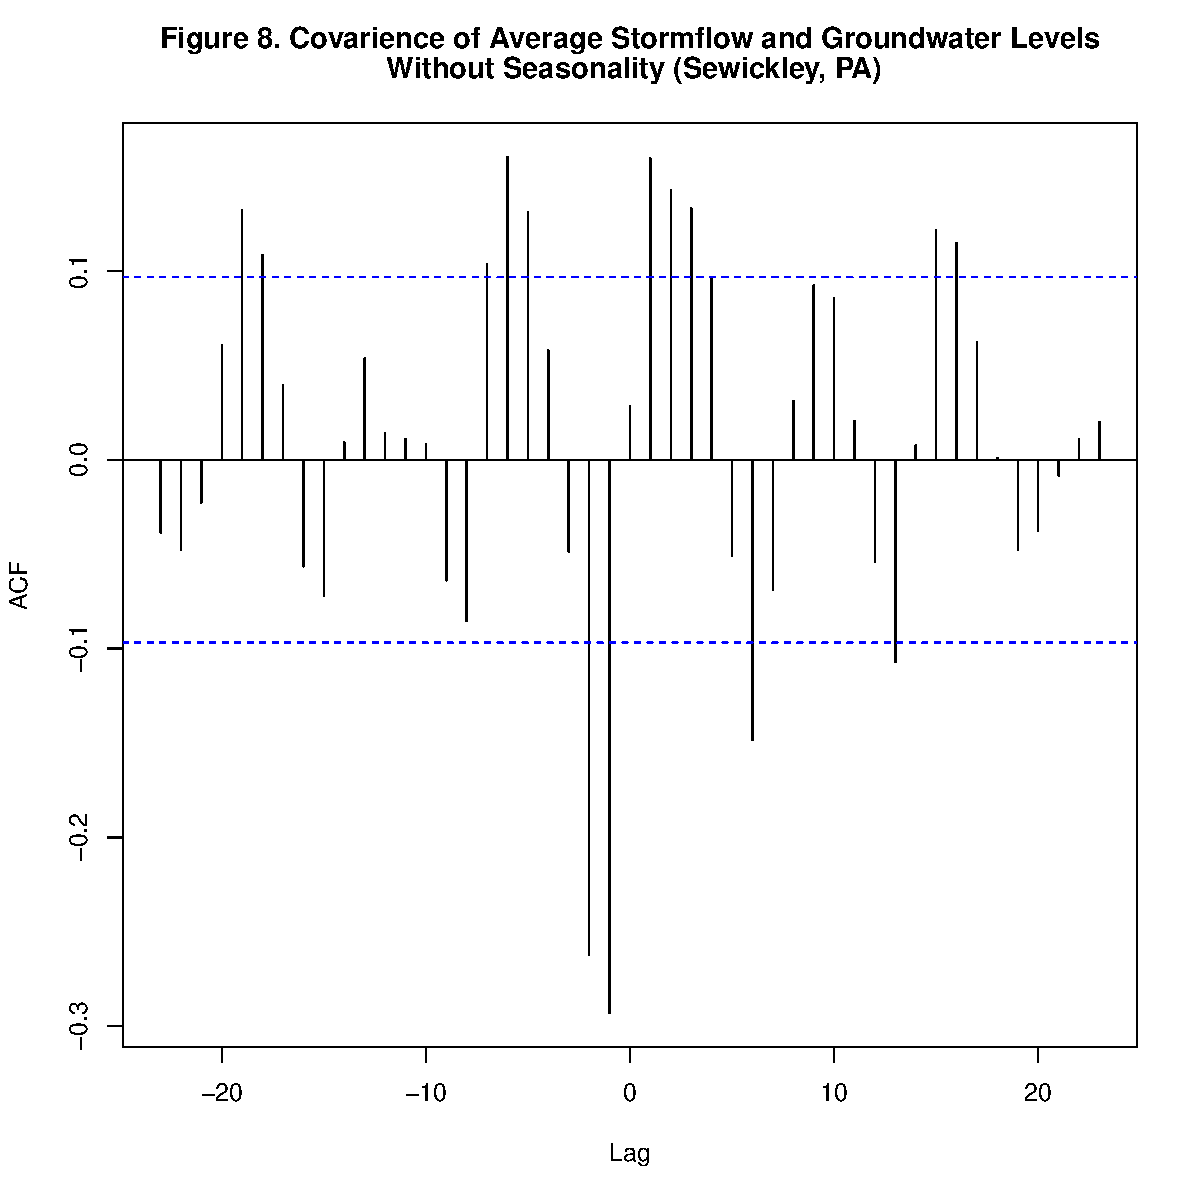
\includegraphics{Draft_Final_files/figure-latex/groundwater_lag-6.pdf}
\newpage

\hypertarget{question-3-how-is-groundwater-quality-changing-overtime-are-chemicals-more-concentrated-at-low-groundwater-levels-or-high}{%
\subsection{Question 3: How is groundwater quality changing overtime?
Are chemicals more concentrated at low groundwater levels or
high?}\label{question-3-how-is-groundwater-quality-changing-overtime-are-chemicals-more-concentrated-at-low-groundwater-levels-or-high}}

Lastly, water quality was analyzed with visual plots and linear
regression. Two of the many available water quality variables were
chosen for analysis: sulfate concentrations and pH. Figures 9 and 10
show how sulfate changes over time and with groundwater depth for
Houserville and Sewickley, PA, respectively. Figure 11 and 12 show how
pH changes over time and with groundwater depth for Houserville and
Sewickley, PA, respectively. Then a linear regression was also run for
sulfate concentration and pH in relation to groundwater level and time
for both sites to test for statistical significance.

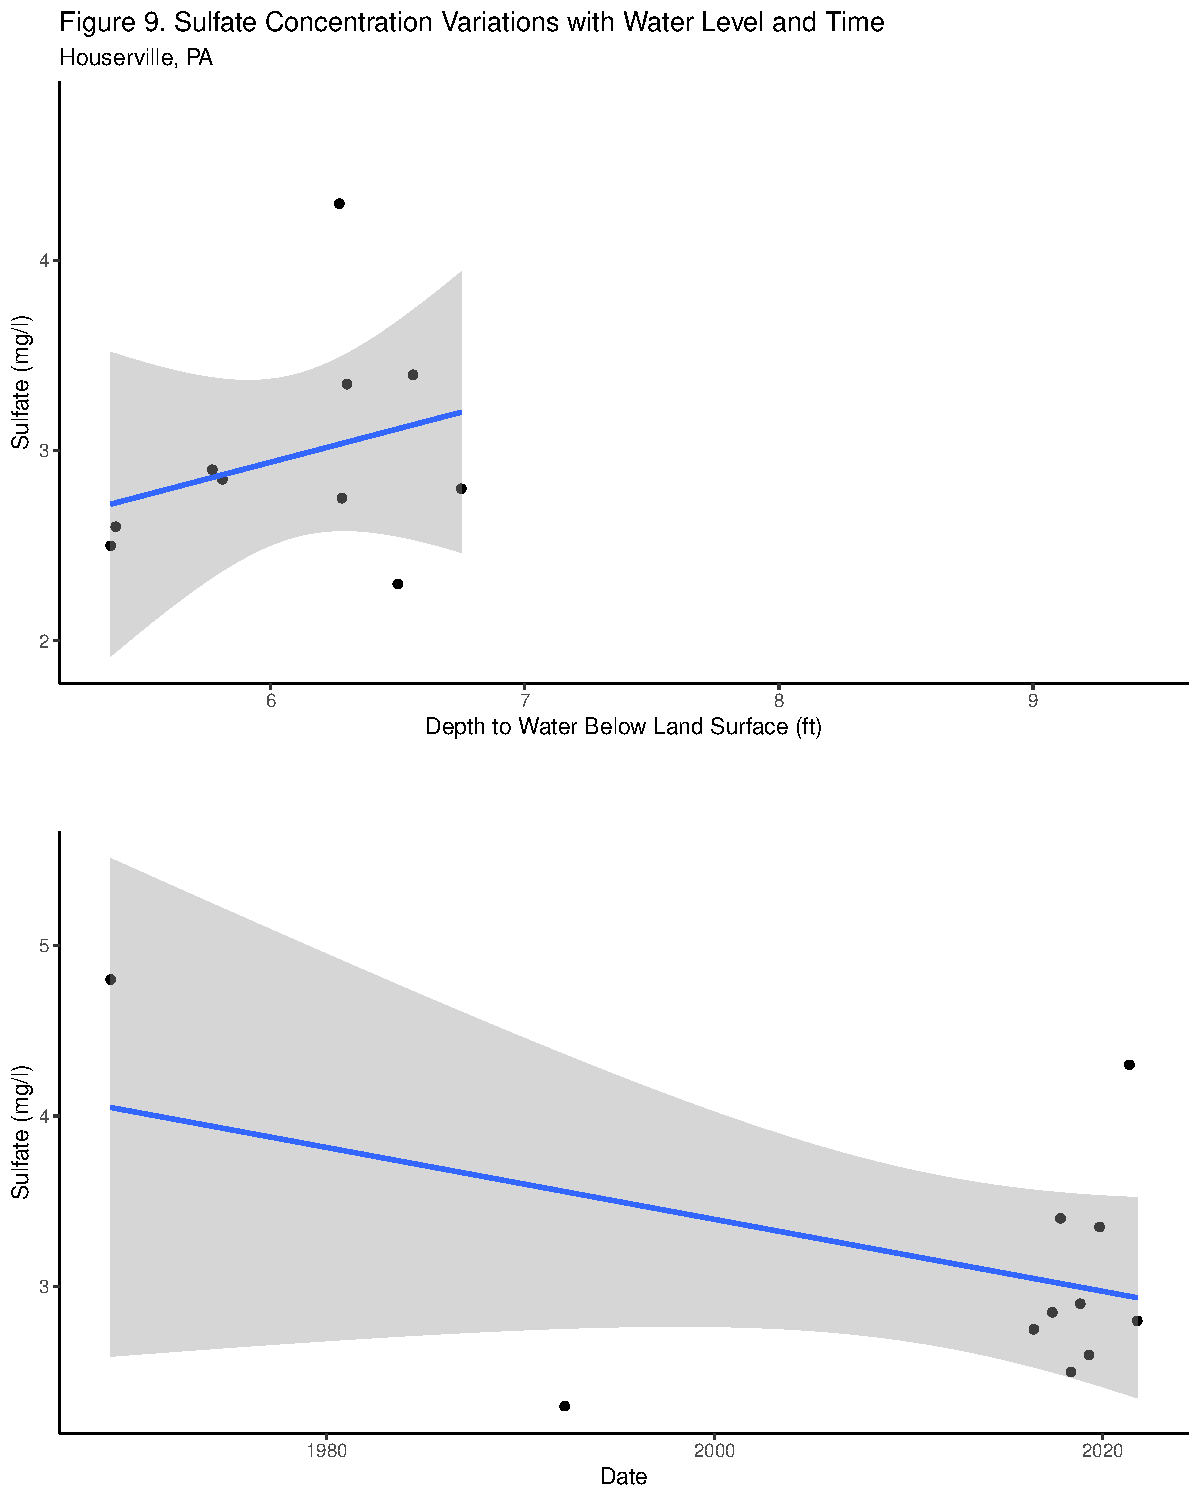
\includegraphics{Draft_Final_files/figure-latex/groundwater_quality-1.pdf}

\newpage

\begin{verbatim}
## 
## Call:
## lm(formula = Sulfate ~ Water_Level, data = groundwater_level_qual_penn)
## 
## Residuals:
##      Min       1Q   Median       3Q      Max 
## -0.81530 -0.27084 -0.07462  0.20793  1.26537 
## 
## Coefficients:
##             Estimate Std. Error t value Pr(>|t|)
## (Intercept)   0.8354     2.4556   0.340    0.742
## Water_Level   0.3508     0.4014   0.874    0.408
## 
## Residual standard error: 0.5852 on 8 degrees of freedom
##   (6 observations deleted due to missingness)
## Multiple R-squared:  0.08713,    Adjusted R-squared:  -0.02698 
## F-statistic: 0.7635 on 1 and 8 DF,  p-value: 0.4077
\end{verbatim}

\begin{verbatim}
## 
## Call:
## lm(formula = Sulfate ~ Date, data = groundwater_level_qual_penn)
## 
## Residuals:
##     Min      1Q  Median      3Q     Max 
## -1.2573 -0.3427 -0.1354  0.3774  1.3560 
## 
## Coefficients:
##                Estimate  Std. Error t value Pr(>|t|)    
## (Intercept)  4.02657793  0.63001574   6.391 0.000127 ***
## Date        -0.00005769  0.00003844  -1.501 0.167624    
## ---
## Signif. codes:  0 '***' 0.001 '**' 0.01 '*' 0.05 '.' 0.1 ' ' 1
## 
## Residual standard error: 0.732 on 9 degrees of freedom
##   (5 observations deleted due to missingness)
## Multiple R-squared:  0.2002, Adjusted R-squared:  0.1113 
## F-statistic: 2.253 on 1 and 9 DF,  p-value: 0.1676
\end{verbatim}

\newpage

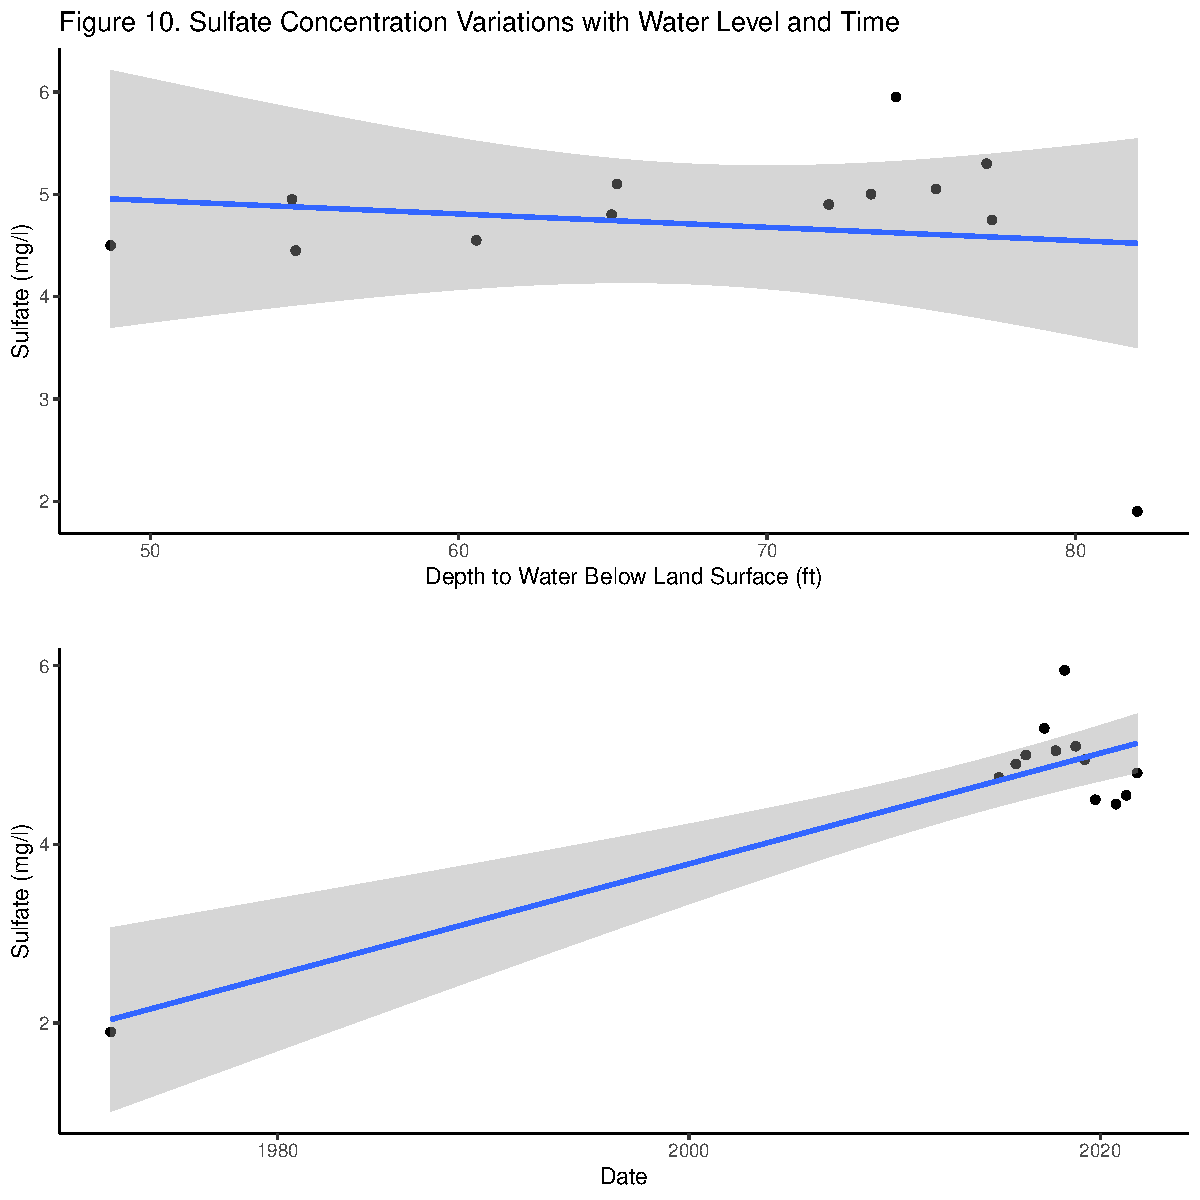
\includegraphics{Draft_Final_files/figure-latex/linear_m2-1.pdf}

\newpage

\begin{verbatim}
## 
## Call:
## lm(formula = Sulfate ~ Water_Level, data = groundwater_level_qual_vr)
## 
## Residuals:
##     Min      1Q  Median      3Q     Max 
## -2.6214 -0.2507  0.1673  0.3662  1.3267 
## 
## Coefficients:
##             Estimate Std. Error t value Pr(>|t|)  
## (Intercept)  5.59012    1.82107    3.07   0.0107 *
## Water_Level -0.01303    0.02661   -0.49   0.6339  
## ---
## Signif. codes:  0 '***' 0.001 '**' 0.01 '*' 0.05 '.' 0.1 ' ' 1
## 
## Residual standard error: 0.9607 on 11 degrees of freedom
##   (3 observations deleted due to missingness)
## Multiple R-squared:  0.02135,    Adjusted R-squared:  -0.06762 
## F-statistic: 0.2399 on 1 and 11 DF,  p-value: 0.6339
\end{verbatim}

\begin{verbatim}
## 
## Call:
## lm(formula = Sulfate ~ Date, data = groundwater_level_qual_vr)
## 
## Residuals:
##      Min       1Q   Median       3Q      Max 
## -0.61873 -0.33288  0.03428  0.16236  1.03622 
## 
## Coefficients:
##              Estimate Std. Error t value  Pr(>|t|)    
## (Intercept) 1.9216772  0.4858293   3.955   0.00225 ** 
## Date        0.0001697  0.0000285   5.955 0.0000952 ***
## ---
## Signif. codes:  0 '***' 0.001 '**' 0.01 '*' 0.05 '.' 0.1 ' ' 1
## 
## Residual standard error: 0.4725 on 11 degrees of freedom
##   (3 observations deleted due to missingness)
## Multiple R-squared:  0.7633, Adjusted R-squared:  0.7417 
## F-statistic: 35.47 on 1 and 11 DF,  p-value: 0.00009519
\end{verbatim}

\newpage

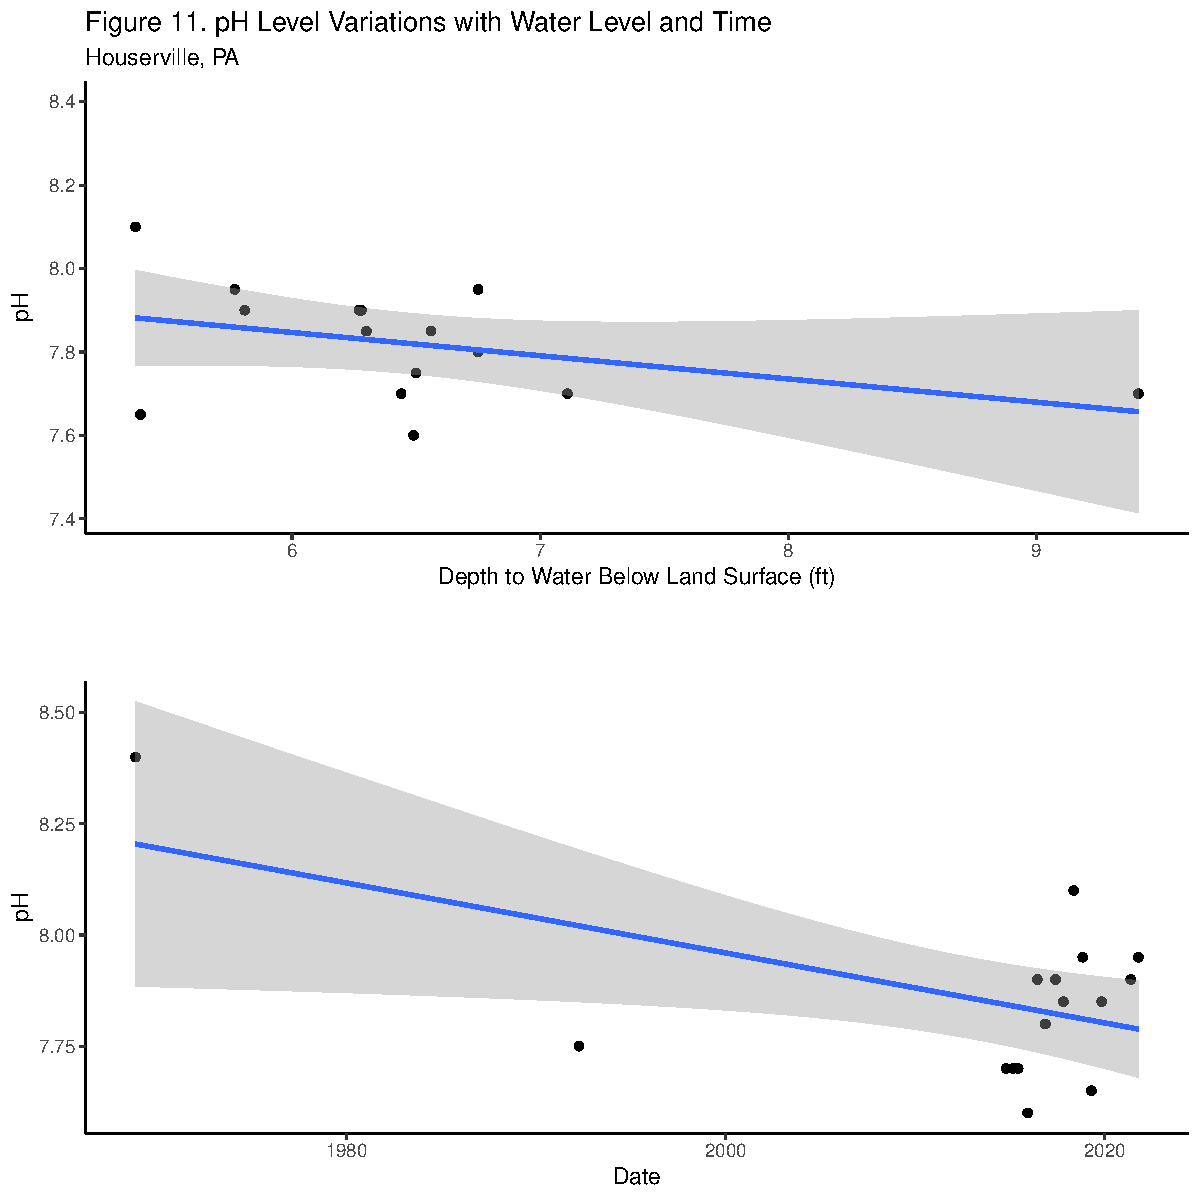
\includegraphics{Draft_Final_files/figure-latex/linear_m4-1.pdf}

\newpage

\begin{verbatim}
## 
## Call:
## lm(formula = pH ~ Water_Level, data = groundwater_level_qual_penn)
## 
## Residuals:
##      Min       1Q   Median       3Q      Max 
## -0.23073 -0.07689  0.03446  0.06858  0.21815 
## 
## Coefficients:
##             Estimate Std. Error t value Pr(>|t|)    
## (Intercept)  8.18106    0.23950  34.159  4.1e-14 ***
## Water_Level -0.05572    0.03659  -1.523    0.152    
## ---
## Signif. codes:  0 '***' 0.001 '**' 0.01 '*' 0.05 '.' 0.1 ' ' 1
## 
## Residual standard error: 0.13 on 13 degrees of freedom
##   (1 observation deleted due to missingness)
## Multiple R-squared:  0.1513, Adjusted R-squared:  0.08606 
## F-statistic: 2.318 on 1 and 13 DF,  p-value: 0.1518
\end{verbatim}

\begin{verbatim}
## 
## Call:
## lm(formula = pH ~ Date, data = groundwater_level_qual_penn)
## 
## Residuals:
##      Min       1Q   Median       3Q      Max 
## -0.27054 -0.14106  0.03836  0.11589  0.28468 
## 
## Coefficients:
##                 Estimate   Std. Error t value Pr(>|t|)    
## (Intercept)  8.195709415  0.145612916  56.284   <2e-16 ***
## Date        -0.000021532  0.000008836  -2.437   0.0288 *  
## ---
## Signif. codes:  0 '***' 0.001 '**' 0.01 '*' 0.05 '.' 0.1 ' ' 1
## 
## Residual standard error: 0.1697 on 14 degrees of freedom
## Multiple R-squared:  0.2979, Adjusted R-squared:  0.2477 
## F-statistic: 5.939 on 1 and 14 DF,  p-value: 0.02875
\end{verbatim}

\newpage

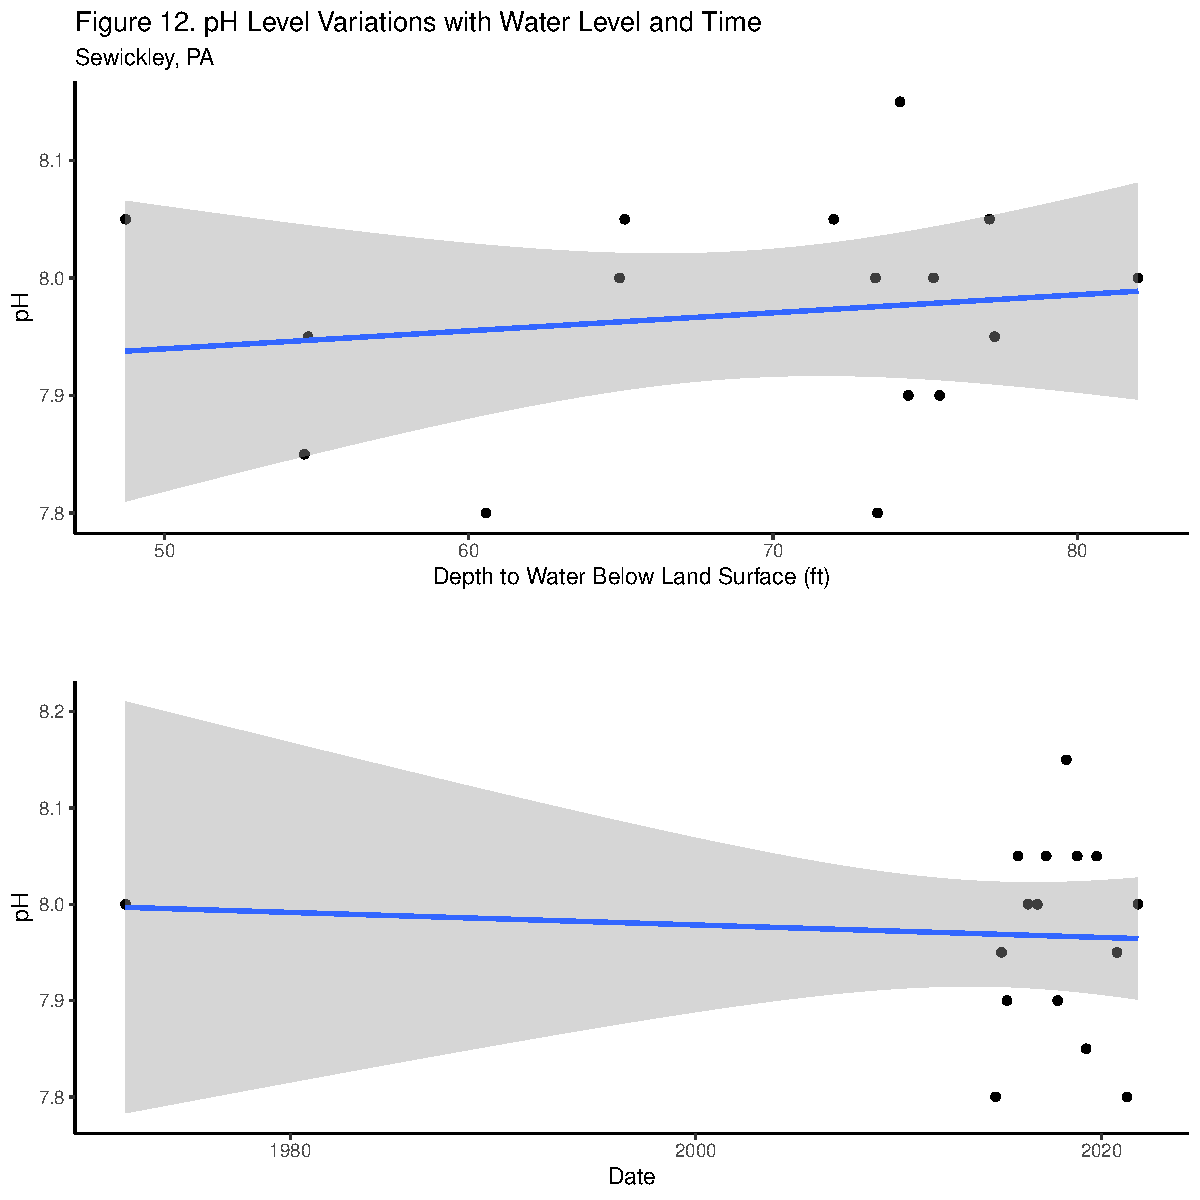
\includegraphics{Draft_Final_files/figure-latex/linear_m6-1.pdf}

\newpage

\begin{verbatim}
## 
## Call:
## lm(formula = pH ~ Water_Level, data = groundwater_level_qual_vr)
## 
## Residuals:
##      Min       1Q   Median       3Q      Max 
## -0.17562 -0.07757  0.01640  0.07070  0.17324 
## 
## Coefficients:
##             Estimate Std. Error t value Pr(>|t|)    
## (Intercept) 7.863025   0.185749  42.332 3.54e-16 ***
## Water_Level 0.001533   0.002669   0.574    0.575    
## ---
## Signif. codes:  0 '***' 0.001 '**' 0.01 '*' 0.05 '.' 0.1 ' ' 1
## 
## Residual standard error: 0.1004 on 14 degrees of freedom
## Multiple R-squared:  0.02303,    Adjusted R-squared:  -0.04676 
## F-statistic:  0.33 on 1 and 14 DF,  p-value: 0.5748
\end{verbatim}

\begin{verbatim}
## 
## Call:
## lm(formula = pH ~ Date, data = groundwater_level_qual_vr)
## 
## Residuals:
##      Min       1Q   Median       3Q      Max 
## -0.16894 -0.06736  0.01763  0.08201  0.18332 
## 
## Coefficients:
##                 Estimate   Std. Error t value Pr(>|t|)    
## (Intercept)  7.998048905  0.103590613  77.208   <2e-16 ***
## Date        -0.000001780  0.000006101  -0.292    0.775    
## ---
## Signif. codes:  0 '***' 0.001 '**' 0.01 '*' 0.05 '.' 0.1 ' ' 1
## 
## Residual standard error: 0.1012 on 14 degrees of freedom
## Multiple R-squared:  0.00604,    Adjusted R-squared:  -0.06496 
## F-statistic: 0.08507 on 1 and 14 DF,  p-value: 0.7748
\end{verbatim}

\newpage

\hypertarget{summary-and-conclusions}{%
\section{Summary and Conclusions}\label{summary-and-conclusions}}

\hypertarget{question-1}{%
\subsection{Question 1}\label{question-1}}

From the analysis, stormflow and groundwater have seasonal trends in
both Houserville and Sewickley, PA. Given this, a seasonal Mann-Kendall
test was run to understand how these variables were changing over time.
In Houserville, stormflow was showing statistical significance for
decreasing over time, while groundwater levels were also decreasing
overtime. In Sewickley, stormflow was showing statistical significance
for decreasing over time, while groundwater levels showed no statistical
significance in trend over time.

\hypertarget{question-2}{%
\subsection{Question 2}\label{question-2}}

Precipitation or in the case of this analysis stormflow should be an
indicator of groundwater levels because groundwater is recharged by
precipitation. In this analysis because groundwater levels are measured
as distance from the ground surface to the water level, the larger the
water level value the less ground water there is. As a result the
relationship for this data is the less stormwater or precipitation there
is the greater the distance is to the water level. When looking at lag
times in Houserville both with and without seasonality there was
statistically significant and most dominant lag was at 0, -21 months.
This means that according to the analysis ground water could be affected
by rainfall within the month or take around 21 months to affect
groundwater levels. For Sewickley there was statistically significant
and most dominant lag at -2 months. This means it takes stormflow or
precip around 2 months to affect groundwater levels. Positively
correlated lag was not considered because that relationship does not
line up scientifically. There is also the possibility that lag could be
seasonal. For example, it could be that as the land is wetter it takes
less time for groundwater to be affected by precipitation.

\hypertarget{question-3}{%
\subsection{Question 3}\label{question-3}}

Lastly, although must of the data was concentrated on recent samples the
most statistically significant finding was that sulfate concentrations
are higher in Sewickley now than before. There is also some evidence in
both Houserville and Sewickley that sulfate concentrations increase as
depth to water below the surface increases. This may suggest that
sulfates are not being flushed out of the system with the water. Most of
the analysis of groundwater quality were statistically insignificant.
More consistent data sampling would be needed to form conclusions.

\newpage

\hypertarget{references}{%
\section{References}\label{references}}

\url{https://cida.usgs.gov/ngwmn/index.jsp}

U.S. Geological Survey, 2016, National Water Information System data
available on the World Wide Web (USGS Water Data for the Nation).

\end{document}
